\section{Petri Nets Considering Time}
	
	In the Ordinary Petri Nets formalism, the time is not consider and this results in indeterminism 
	regarding the time. It is not specified when a sensibilized transition will be fired or even if it
	will be fired. Neither can be said which transition from a group of transitions in conflict will 
	be fired \cite{garciaizquierdo}.
	
	There are three different interpretations about how the time should be consider. All of them have 
	focus on reduce the indeterminism regarding time in Petri Nets.
	\begin{enumerate}
	  	\renewcommand{\theenumi}{\Alph{enumi}}
	  	\item \underline{Stochastic Petri Net}
	  		\\
			Introduces a stochastic estimation on the instant of firing of a transition.
		\item \underline{Timed Petri Net}
			\\
			Introduces a time condition which specifies the duration of the transition.
		\item \underline{Time Petri Net}
			\\
			Introduce temporary dimensions between which the transition should be fired.
	\end{enumerate}
		
	\begin{figure}[h]
		\centering
		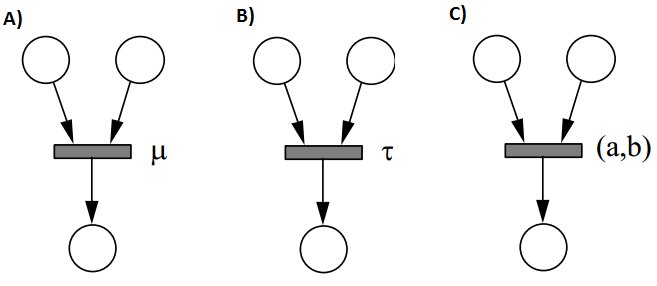
\includegraphics[width=1\linewidth]{./img/Petri16}
		\caption{Different ways to intruduce time in Petri Nets}
		\label{fig:Petri16}
	\end{figure}
	
	The temporal parameters associated with transitions can be interpreted in these three different
	ways\footnotemark:
	
	\footnotetext{ $\bullet t$ is the set of places that are inputs to a
	transition, mathematically defined as: $\bullet t = \{ p \in P : (p , t) \in F \}$.
	
	$t \bullet$ is the set of positions that are outputs of a transition, mathematically defined as: 
		$t \bullet = \{ p \in P : (t , p) \in F \}$.
	
	$F$ is the set of arcs, input and output to the transitions-
	}	
	
	\begin{enumerate}
	  	\item Generalised Stochastic Petri Nets (GSPNs) \cite{gspn} have two different types of 
	  		transitions: immediate transitions and timed transitions. When a transition \emph{t} is
	  		sensitized, its firing could be:
			\begin{enumerate}
			  	\item with a duration equal to zero if the transition \emph{t} is immediate.
			  	\item after lapse of a random time. This random time is expressed by an exponential 
			  	distribution. The A net from the figure \ref{fig:Petri16} graphically represents an stochastic
			  	timed transition where its probability to be fired is represented by $\mu$.
			\end{enumerate}
		\item Timed Petri Nets have two different types of transitions: immediate transitions and timed
			transitions. When a transition \emph{t} is sensitized, its firing could be:
			\begin{enumerate}
			  	\item with a duration equal to zero if the transition \emph{t} is immediate.
			  	\item with immediate removal of tokens from $\bullet t$ set but placing the tokens in 
			  	the $t \bullet$ that only after time $\tau$ has elapsed. Meanwhile, the transition 
			  	can not be sensitized. The B net from the figure \ref{fig:Petri16} graphically represents 
			  	a timed transition with a delay equal to $\tau$.
			\end{enumerate}
		\item Timed Petri Nets have two different types of transitions: immediate transitions and time
			transitions. When a transition \emph{t} is sensitized, its firing could be:
			\begin{enumerate}
			  	\item with a duration equal to zero if the transition \emph{t} is immediate.
			  	\item if it is a time transition, at the time it is sensitized, a timer stars. The transition
			  	can only be fired when the timer value is between the limits of the interval [a, b].
			  	Otherwise, the transition can not be fired. Once the firing was performed, the timer is
			  	restarted. The C net from the figure \ref{fig:Petri16} graphically represents  a time transition
			  	with an associated interval equal to [a, b].
			\end{enumerate}		
	\end{enumerate}
	
	Should be noted that all the firings are performed in two steps.
	\begin{enumerate}
		\item The removal of the tokens from the $\bullet t$ set. This is an atomica action and the amount
			of tokens removed from each place is equal to the weight of the arcs joining each place $p \in
			\bullet t$ with the transition $t$.
		\item The atomic action of placing in each place of $t \bullet$ set the amount of tokens indicated
			by the weight of the arcs joining each place $p \in t \bullet$ with the transition $t$..
	\end{enumerate}
	